\documentclass[letterpaper,11pt]{article}

\usepackage{booktabs}

\usepackage{amsmath,amssymb,amstext,amsthm} % Lots of math symbols and environments
\usepackage[pdftex]{graphicx} % For including graphics N.B. pdftex graphics driver 

%custom packages
\usepackage[usenames,dvipsnames,svgnames,table]{xcolor}
\usepackage[greek,english]{babel}
\usepackage{cancel}
\usepackage{comment}
\usepackage{courier}
\usepackage{fixltx2e}  % for subscript text in sections/bookmarks
\usepackage[top=1in, bottom=1in, left=1in, right=1in]{geometry}
\usepackage{listings}
%\usepackage[12pt]{moresize}
\usepackage{multirow}
\usepackage{tikz}
%\usepackage{ulem}
\usepackage{url}
\usepackage[utf8]{inputenc}

% Theorem Styles
\newtheorem{theorem}{Theorem}[section]
\newtheorem{lemma}[theorem]{Lemma}
\newtheorem{proposition}[theorem]{Proposition}
\newtheorem{corollary}[theorem]{Corollary}
% Definition Styles
\theoremstyle{definition}
\newtheorem{definition}{Definition}[section]
\newtheorem{example}{Example}[section]
\theoremstyle{remark}
\newtheorem{remark}{Remark}

% Code Styles
\newcommand{\und}{\char`_}
\newcommand{\cdf}{\bf\ttfamily} % code font and family
\newcommand{\cde}{\cdf\footnotesize}  % basic listing style
\newcommand{\cd}{\cdf\small}  % basic inline-code style
\lstdefinelanguage{ScalaExamples}{
	morekeywords={
		def,var,val,type,object,package,class,abstract,trait,extends,with,
		match,case,
		import,
		this,super,override,
		private,protected,public,
		final,sealed,null,new,
		for,do,while,until,yield,return},
	sensitive=true,
	morecomment=[l]{//},
	morecomment=[s]{/*}{*/},
	morestring=[b]"
}
\lstset{
	language={ScalaExamples},
	basicstyle=\cde,
	tabsize=2,
	keywordstyle=\cde\color{Blue},
	identifierstyle=\cde,
	commentstyle=\bf\scriptsize\color{gray},
	%xleftmargin=\parindent,
	extendedchars=true,
	breaklines=true,
	captionpos=b,
	frame=b,
	float=htp,
	emph={@pure,@readonly,@mutable,@polyread},
	emphstyle={\cde\color{OliveGreen}},
	moredelim=**[is][\cde\color{OliveGreen}]{@*}{*@},
	escapeinside={(*}{*)}
}

% Overline
% Credit: http://tex.stackexchange.com/questions/24132/overline-outside-of-math-mode
\makeatletter
\newcommand*{\ovr}[1]{$\overline{\hbox{#1}}\m@th$}
\makeatother

\begin{document}

\title{Reference Immutability for Scala}
\author{Jonathan Rodriguez\\University of Waterloo}
\maketitle


The theory in this case is that the proposed process/approach yields ``better'' progress toward an ``important'' goal.
``Better'' is normally defined across a number of relevant dimensions.
``Important'' is motivated intrinsically or extriniscally.
Intrinsic importance is subjective, and the only way to get such work published is to persuade (or come to an agreement with) others about the intinsically interesting nature of the topic. (There is no such thing as objectively interesting work. Interest is always subjective--the work is interesting to whom?)


The real question we want to answer here is:
What aspects of the proposed system are worth further investigation or implementation?


Utility dimensions for programmer-friendly side-effect limitation systems
\begin{itemize}
\item{\bf Utility.} How useful is the knowledge expressed by the annotations? (What can be done with that knowledge?)

\item {\bf Consistency.} Is it possible to compile and run code with inconsistent annotations? If so, how easy is it to unintentionally introduce unchecked inconsistencies?

\item {\bf Ease of Learning.} Will it be easy for the target programmer to learn the meanings of the annotations and use those annotations effectively?

\item {\bf Code Restructuring.} Does fully-annotated code require substantial refactoring, or can typical code be fully annotated as-is? (To define: ``fully annotated'')

\item{\bf Compatibility with Existing Code.} Does enabling the new feature break compatibility with existing code? If so, how much backward compatibility is lost?

\item {\bf Visual Complexity.} Are the annotations easy or difficult to parse visually?

\item {\bf Annotation Density.} Does fully-annotated code tend to require many or few annotations? (Inference reduces this.) (``Annotations required'' in the present work also includes new type annotations.)

\item {\bf Incremental Annotation Burden.} Const hell. Annotation of the standard library.

\item{\bf Computational Efficiency.} Is compiling annotated code substantially slower than compiling unannotated code? Does enabling the new feature slow down compilation of existing unannotated code?

%\item Easy to replicate or reimplement the idea. (?)
\end{itemize}

Do the annotations tend to obscure the meaning of the underlying code?
The answer to this question is likely a combination of annotation density, visual complexity, and ease of use (improper use could obfuscate code more easily).

% Whaat do union types have to do with the evaluation?


The context of this work is ``Scala-like'' languagues.

The formulation of the work involves type unions and intersections, a novel method of representing reference immutability.

The soundness problem is dealt with in the following way:
the purity problem becomes a reference immutability problem,
which becomes a type soundness problem.

I expect the proposed approach to be visually lightweight.
The lightweightness of the system is expected to be supported by Scala's local type inference features.
JPure has quite clear and lightweight annotations, as do other RI systems, so I expect this system to maintain the lightweightness.



% Interest

% Topic
Reference immuability and side-effect limitations.

% The Question(s) I plan to answer here: ...
What is a reasonable way to help programmers statically reason about possible side effects in Scala-like languages?
What can I say about the reusability of the type system/inference? (How useful are union/intersection types? Are the benefits/drawbacks to using automatic type inference?) What about extensibility problems?

% What's the theory (tentative answer to the question)?
% The theory here is about an idea, or a system of related ideas (which is itself an idea), and the answer is about utility of the idea with respect to a particular purpose.
Reference immutability permissions can be represented as type unions and intersections.
Mutability may be understood as a permission that can be added to or removed from arbitrary types by means of type unions and intersections.

% Implementation

% Methodology: what do we mean by "reasonableness," and how can we practically evaluate it? (not all dimensions can be evaluted to the nth degree, so we get picky about it)
% dimensions

% What (precisely) we're going to measure

% How we're going to measure



% General comments
% "Novelty" from a research perspective is just a way of saying that we have not considered (or considered as thoroughly) the given question.
% In CS, theories take the form, "If one does X rather than Y in a given context C, then one is likely to obtain the range Z of relative advantages and disadvantages."
% So there is a measurement of agency involved; either a human is doing X or Y, or a machine is.
% There is also a repeatability involved in theformulation of this theory: we are not asking about nonrepeatable actions; we are asking about actions performed within a context that is general enough that others can use your research to inform their own actions.
% Sometimes there is no explicit comparision of approaches. Instead, the paper is of the form, "We did X, and Z happened." This is fine under the condiiton that X has not been done before (so we have no prior information about X).
% The rigour of the comparision element should be related to the importance of the question: a rigourous comparision between actions that nobody cares about is probably a waste of time.

% Incremental annotation burden?
% "Near-maximal typings" with few annotations?
% Precision: difficulty of expressing purity where purity exists?

%\subsection{Discussion of the Area and its Methodologies}

% The motivations for studies in the programming languages area seem to me to be roughly categorizable into two distinct groups.
% The motivations in the first group of studies are to improve the functionality of a software system by means of optimization of compute time, memory use, or other resource.
% For example, 

% The motivations for studies in the programming languages area seem to me to be categorizable into two distinct groups. Studies in the first group are aimed at improving performance, memory usage, or power usage. I will refer to this group as ``intra-system'' studies. Intra-system studies take the human interface elements and language standards as a given, and attempt to improve functionality in 

% Studies in the second group are aimed at improving the human usability, flexibility, and application of the system. The interface between the human and the machine 


% Occam's Razor, parsimony: the solution(s) presented here is(are) candidates for the simplest answer(s) to the given question(s)

% study at the intimation of Providence?
% Yes.


%\subsubsection{}


\section{Mutability and Types}


\subsection{Mutability as a Permission}

Logically, it is possible to represent mutability as a {\em permission tag} that may be present as a type member. See listing~\ref{lst:mutability-as-tag} for a hypothetical example. On the left, there is a type containing a single declared member {\cd foo}. On the right, there is a type containing both {\cd foo} and the permission tag {\cd <mutable>}.

The presence of a permission tag on a type allows certain operations to be performed on objects of that type, and conversely, the absence of a permission tag prevents certain operations from being performed. Specifically, the absence of the {\cd <mutable>} permission on type {\cd T1} prevents assignment to any field of an object typed {\cd T1}, and it also prevents any read of such a field from returning a reference that contains the {\cd <mutable>} permission.

\begin{lstlisting}[float=htbp, caption={Mutability as a Permission Tag}, label={lst:mutability-as-tag}]
Type Without Mutability Permission     Type With Mutability Permission
----------------------------------     -------------------------------
type T1 = {                            type T2 = {
  var foo: U                             var foo: U
}                                        permission <mutable>
                                       }
\end{lstlisting}

The right type~{\cd T2} is a subtype of the left type~{\cd T1}, at least under a structural typing regime. (Under a nominal regime, we may not be able to determine this particular subtype relationship because {\cd T1} and {\cd T2} are not related by inheritance. However, the approximations made by a nominal regime are not relevant to the present discussion.)

%The presence of the {\cd <mutable>} permission on type {\cd T2} increases the size of the set of possible operations that are safe to perform relative to {\cd T1}, and since an increase in the number of safe operations generally indicates a more specific type, we can reasonably say that {\cd T2} is a subtype of {\cd T1}.

\subsection{Mutability as a Trait}

Rather than implementing the mutability permission literally as a type member, in the present work I explore the possibility of implementing the mutability permission as a trait/mixin.
The {\cd MutableAny} trait represents the presence of the mutability permission, and mutability can be added to any type by means of {\em type intersection}. Type intersection in Dotty can be done with either the {\cd with} keyword or the amperstand type-intersection operator {\cd \&}.
For example, listing~\ref{lst:intersection-mutableany} shows two ways of defining a type~{\cd U} as a mutable version of type~{\cd T}.
Type~{\cd U} logically contains all of the same members as type~{\cd T}, as well as the mutability permission.

\begin{lstlisting}[float=htbp, caption={Intersection with MutableAny}, label={lst:intersection-mutableany}]
type U = T with MutableAny
type U = T & MutableAny
\end{lstlisting}

Type intersection is the basic mechanism for adding mutability permissions to a type.

\subsection{Revoking Mutability Permissions}

It is sometimes necessary to build types where mutability permissions have been revoked.
The revocation of mutability is done by means of a {\em type union}, which is expressed in Dotty by the vertical-bar type-union operator~{\cd |}, as in listing~\ref{lst:union-readonlynothing}.

\begin{lstlisting}[float=htbp, caption={Union with ReadonlyNothing}, label={lst:union-readonlynothing}]
type U = T | ReadonlyNothing
\end{lstlisting}

The {\cd ReadonlyNothing} trait requires some explanation. {\cd ReadonlyNothing} is assumed to contain all possible members, except for the mutability permission. The type union operation preserves only those members that are common to both operands, so type~{\cd U} in listing~\ref{lst:union-readonlynothing} contains exactly the set of members as type~{\cd T}, except for the mutability permission.

\subsection{Default Mutabilities} \label{sec:default-mutabilities}

Most types are considered mutable by default.

The only types that are not mutable by default are {\cd Any} and {\cd ReadonlyNothing}.
The non-mutability of {\cd ReadonlyNothing} is self-explanatory, but the non-mutability of {\cd Any} requires some explanation.

In a cursory examination of practical code, I have seen three dominant uses of {\cd Any}: first, as the upper bound of an abstract type parameter; second, as the type of a method parameter that may be dynamically downcast within the method; and third, as the element type of a container. Listing~\ref{lst:dominant-uses-of-any} shows examples of these uses.

\begin{lstlisting}[float=htbp, caption={Dominant Uses of the Any Type}, label={lst:dominant-uses-of-any}]
class List[E] { ... }                         // Case 1

def m(x: Any) = x match { case x: T => ... }  // Case 2

val map: Map[String, Any]                     // Case 3
\end{lstlisting}

In case~1, the abstract type parameter~{\cd E} is not assigned an explicit upper bound, so a default upper bound of {\cd Any} is assumed. In case~2, the method parameter~{\cd x} is dynamically cast to a subtype before any possibly-mutating methods are called. In case~3, {\cd Any} is used as an opaque type, allowing storage and retrieval of arbitrary objects. In none of these cases is a mutating method called directly on an object with type {\cd Any}.

The only potentially problematic case is case~2, where {\cd Any} is downcast to another type.
If {\cd Any} is assumed to be {\em readonly}, then preservation of static reference-immutability guarantees requires that all downcasts of~{\cd x} are also readonly.
Otherwise, a downcast may unintentionally permit a mutation that should have been prohibited.

An alternative is to consider {\cd Any} to be a mutable type, and introduce a different (readonly) top type. Unfortunately, there is a pervasive assumption in the Dotty compiler that {\cd Any} is the top type. Attempting to change this assumption to support case~2 code examples seemed like it would create more problems than it would solve.

Ideally, the type of parameter~{\cd x} in case~2 would be {\cd MutableAny} rather than {\cd Any}. In practice, generating errors for code like case~2 would force programmers to perform the replacement of {\cd Any} by {\cd MutableAny} manually, unless some kind of automatic replacement is done.

It is possible to automatically substitute explicit uses of {\cd Any} with {\cd MutableAny} at compile time, which will perhaps go most of the way toward allowing legacy code to compile as-is. Such a substitution would affect the uses of {\cd Any} in cases~2 and~3, but not the default upper bound of type parameter~{\cd E} in case~1.

\subsection{Type Lattice}

The default Dotty type lattice is as shown in figure~\ref{fig:default-type-lattice}. {\cd Any} is a supertype of all other types, and {\cd Nothing} is a subtype of all other types.

\begin{figure}[htbp]
\center
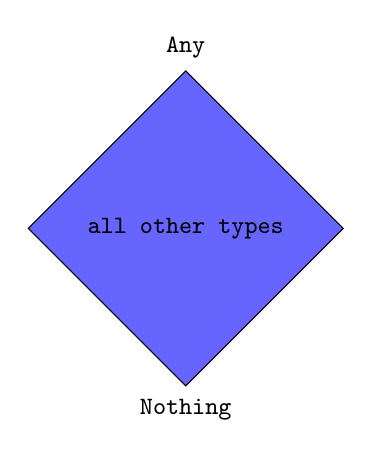
\begin{tikzpicture}
	\filldraw[fill=blue!60, draw=black] (0, 2) -- (2, 0) -- (0, -2) -- (-2, 0) -- cycle;
	\draw (0, 2.3) node{\cd Any};
	\draw (0, 0) node{\cd all other types};
	\draw (0, -2.3) node{\cd Nothing};
\end{tikzpicture}
\caption{Default Type Lattice}
\label{fig:default-type-lattice}
\end{figure}

\begin{figure}[htbp]
\center
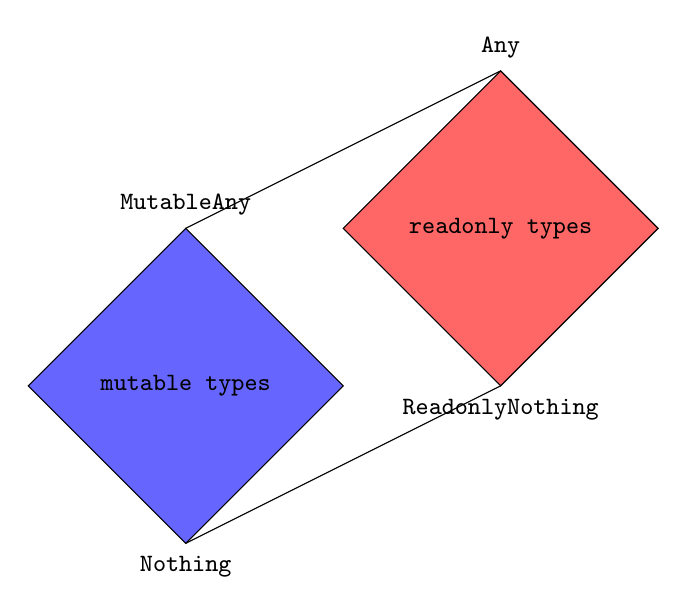
\begin{tikzpicture}
	\filldraw[fill=red!60, draw=black] (0, 2) -- (2, 0) -- (0, -2) -- (-2, 0) -- cycle;
	\draw (0, 2.3) node{\cd Any};
	\draw (0, 0) node{\cd readonly types};
	\draw (0, -2.3) node{\cd ReadonlyNothing};

	\filldraw[fill=blue!60, draw=black] (-4, 0) -- (-2, -2) -- (-4, -4) -- (-6, -2) -- cycle;
	\draw (-4, 0.3) node{\cd MutableAny};
	\draw (-4, -2) node{\cd mutable types};
	\draw (-4, -4.3) node{\cd Nothing};

	\draw[black] (-4, 0) -- (0, 2);
	\draw[black] (-4, -4) -- (0, -2);
\end{tikzpicture}
\caption{Type Lattice with Mutability}
\label{fig:type-lattice-with-mutability}
\end{figure}

When mutability is added, the lattice is extended to include two versions of each type: one with the mutability permission, and one without. For every mutable type, there is a readonly supertype that is identical except for the absence of the mutability permission. Figure~\ref{fig:type-lattice-with-mutability} shows the extended lattice graphically.

Legacy code assumes the type lattice shown in figure~\ref{fig:default-type-lattice}. The relationships in the lower diamond of figure~\ref{fig:type-lattice-with-mutability} (the ``mutable types'') are identical to the relationships in the ``all other types'' diamond of figure~\ref{fig:default-type-lattice}, allowing legacy code to compile cleanly (modulo some special handling of the {\cd Any} type, as discussed in section~\ref{sec:default-mutabilities}).

The distinction between {\cd Nothing} and {\cd ReadonlyNothing} is important. Most types represent the {\em presence} of members or permissions, but {\cd ReadonlyNothing} represents the {\em absence} of a permission. The idea of using {\cd Nothing}-like types to express the absence of members may be worth exploring further in future work. In the present work, I restrict investigation of {\cd Nothing}-like types to the use of {\cd ReadonlyNothing} for permission removal.

%Although it is not possible to construct an object of either type, 

%It is not possible to construct an object of type {\cd Nothing}, nor is it possible to construct an object of type {\cd ReadonlyNothing}. 

\subsection{Viewpoint Adaptation of Fields}

Type unions and intersections are used to perform viewpoint adaptation of field reads.
Given a reference~{\cd t} of type~{\cd T}, and a field~{\cd u} of type~{\cd U}, the type of \mbox{\cd t.u} is:
\begin{figure}[h]
\center
{\cd T \& ReadonlyNothing | U}
\caption{Viewpoint Adaptation (Field Type {\cd U} with Prefix Type {\cd T})}
\label{fig:viewpoint-adapted-type}
\end{figure}

The expression \mbox{\cd T \& ReadonlyNothing} produces the greatest lower bound of~{\cd T} and {\cd ReadonlyNothing}. Referring the the type lattice in figure~\ref{fig:type-lattice-with-mutability}, the lower bound of~{\cd T} and {\cd ReadonlyNothing} is minimally {\cd Nothing} and maximally {\cd ReadonlyNothing}. The minimal result {\cd Nothing} occurs where~{\cd T} is mutable, and the maximal result {\cd ReadonlyNothing} occurs where~{\cd T} is readonly. The expression {\cd T \& ReadonlyNothing} is therefore a way to ``extract'' the mutability permission from~{\cd T} while ignoring all other members of~{\cd T}.

The subsequent union with type~{\cd U} finds the least upper bound of \mbox{\cd T \& ReadonlyNothing} and~{\cd U}. The result is minimally just~{\cd U}, and maximally \mbox{\cd ReadonlyNothing | U}, which is equivalent to~{\cd U} without any mutability permission.

The viewpoint adaptation formula in figure~\ref{fig:viewpoint-adapted-type} protects the transitive reference-immutability guarantee.
The mutability of the viewpoint-adapted type is the least upper bound of the mutabilities of~{\cd T} and~{\cd U}, which means that it cannot be less restrictive with respect to mutability than either~{\cd T} or~{\cd U}.

\subsection{Mutability Extraction and Assignment}

Type unions and intersections are also used to ``extract'' the mutability of any given type.
Figure~\ref{fig:mutability-of-type} shows the extraction of the mutability portion of an arbitrary type~{\cd T}.
Note that the formula given in figure~\ref{fig:mutability-of-type} is essentially a viewpoint adaptation of {\cd MutableAny} with a prefix type~{\cd T}.

\begin{figure}[h]
\center
{\cd T \& ReadonlyNothing | MutableAny}
\caption{Mutability of a Type}
\label{fig:mutability-of-type}
\end{figure}

Mutability can also be ``assigned'' to a type as shown in figure~\ref{fig:assigning-mutability-to-type}.
Type~{\cd M} is an arbitrary mutability type, with a lower bound of {\cd MutableAny}. Type~{\cd M} may be 
The union with {\cd ReadonlyNothing} produces {\cd T} without any mutability permissions, and the subsequent intersection with {\cd M} adds the desired permissions.

\begin{figure}[h]
\center
{\cd (T | ReadonlyNothing) \& M} \\
\caption{Assigning Mutability {\cd M} to a Type {\cd T}}
\label{fig:assigning-mutability-to-type}
\end{figure}

By combining mutability extraction and assignment, it is possible to create type with the mutability of a different type. In figure~\ref{fig:assigning-mutability-to-type-2}, a type with the members of {\cd T} and the mutability of {\cd U} is created.

\begin{figure}[h]
\center
{\cd U \& ReadonlyNothing | T} \hspace{0.4cm} (where {\cd T} is mutable) \\
{\cd (T | ReadonlyNothing) \& (U \& ReadonlyNothing | MutableAny)} \hspace{0.4cm} (general case) \\
\caption{Creating a Type with the Mutability of a Different Type}
\label{fig:assigning-mutability-to-type-2}
\end{figure}

The ``building blocks'' of viewpoint adaptation, mutability extraction, and mutability assignment are used to flexibly express reference immutability in a wide variety of code situations.



\begin{comment}

\subsection{Identities}

Some useful identities are shown in figure~\ref{lst:}. 

\begin{figure}[h]
\center
{\cd T | ReadonlyNothing} \\

\caption{Identities}
\label{fig:assigning-mutability-to-type-2}
\end{figure}


\subsection{Polymorphic Mutability}

Sometimes it is advantageous to express that a type is polymorphic in its mutability.

\begin{lstlisting}[float=htbp, caption={Union with ReadonlyNothing}, label={lst:union-readonlynothing}]
// Monomorphic method signature
def m(x: S): U

// Method signature with polymorphic mutability
def m[P >: MutableAny](x: (S | ReadonlyNothing) & P): (U | ReadonlyNothing) & P
\end{lstlisting}

\begin{lstlisting}
Is it reasonable to override:
	def f[P >: MutableAny](this: (S | ReadonlyNothing) & P): (U | ReadonlyNothing) & P
with:
	val f: U
The question is whether this.f for either case is compatible?
\end{lstlisting}

\begin{lstlisting}
Let f be a member of x, and let the type of f be U.
1. Let the type of x be S.

	The type of x.f is: S & ReadonlyNothing | U

2. Let the type of x be (S | ReadonlyNothing) & P.

	The type of x.f is: (S | ReadonlyNothing) & P & ReadonlyNothing | U

\end{lstlisting}


%---

% let T = (S | ReadonlyNothing) & P
% let f in x and f: U
% the type of t.u is T & ReadonlyNothing | U

% the type of the return of m is (U | ReadonlyNothing) & P
% big question: is T & ReadonlyNothing | U <: (U | ReadonlyNothing) & P ?  Or are they equal ?

% T & ReadonlyNothing | U <: (U | ReadonlyNothing) & P
% (S | ReadonlyNothing) & P & ReadonlyNothing | U <: (U | ReadonlyNothing) & P
% (S | ReadonlyNothing) & P & ReadonlyNothing | U <: U & P | ReadonlyNothing & P
% S & P & ReadonlyNothing | P & ReadonlyNothing | U <: U & P | ReadonlyNothing & P
% U | S & P & ReadonlyNothing | P & ReadonlyNothing <: P & U | P & ReadonlyNothing
% U | P & ReadonlyNothing <: P & U | P & ReadonlyNothing

% ?  is U | (ReadonlyNothing & P) == (U | ReadonlyNothing) & P  ?

\subsubsection{Discussion of Alternatives: Dynamic Permissions}

The focus of the present work is on static checking of mutability permissions, but an alternative direction would have been to provide dynamic support for mutability permissions. Although I do not implement or evaluate dynamic mutability permissions in the present work, the idea is perhaps worth a very brief discussion.

\begin{lstlisting}[float=htbp, caption={Permission Tag Example}, label={lst:permission-tag-example}]
type T2 = {
	var foo: T2 = this
	permission <mutable>
}
type T1 = {
	var foo: T2 = this
}
val t = new T2()
t.foo                      // result contains permission <mutable>
t.asInstanceOf[T1]         // result does not contain permission <mutable>
t.asInstanceOf[T1].foo     // result does not contain permission <mutable>
\end{lstlisting}

Normally, the type of an object is fixed at the time it is created. However, where there is viewpoint adaptation, the observed type of an object depends on the path used to reach that object.

Consider listing~\ref{lst:permission-tag-example}. The reference~{\cd t} refers to a new object that has the {\cd <mutable>} permission. However, if {\cd t} is cast to type {\cd T1} (which is reasonable in a structural regime if not necessarily a nominal one), the type of the resulting reference cannot contain the {\cd <mutable>} permission. Furthermore, 


It is possible that the path-dependence of viewpoint adaptation may be related in some way to the path-dependence of DOT. However, I do not elaborate further on this thought in the present work.

% Translation of mutability permissions into traits/mixins.



The fundamental approach I take here is to treat mutability as a {\em permission} represented by a {\em trait} or {\em mixin}. By representing mutability as a trait, mutability can be added to any type by means of type intersection.

Practically, I introduce a the trait {\cd MutableAny} to represent the presence of the mutability permission. Given any arbitrary type {\cd T}, the mutability permission can be added using either the {\cd with} keyword or the amperstand ({\cd \&}) type intersection operator:

\begin{lstlisting}
type U = T with MutableAny
type U = T & MutableAny
\end{lstlisting}

In either case, the resulting type~{\cd U} is understood to contain all declarations in {\cd T}, as well as the mutability permission. It is reasonable to understand the mutability permission as a declaration that may be present in a type (other kinds of declarations allowed in Dotty are fields, methods, and type members). I did not literally implement permissions as a fourth kind of declaration in Dotty. Although the permission-as-declaration concept is an intriguing possibility for future study, it is too complex of a topic to discuss thoroughly in the present work.

In the present work, {\cd MutableAny} is assumed to contain the mutability permission. Other named classes and traits are also assumed to contain the mutability permission, for the purpose of allowing existing code to compile without modification. The only exception is the top type {\cd Any}, which is {\em not} assumed to contain the mutability permission. Before moving on, I discuss the rationale and tradeoffs involved in the choice to treat {\cd Any} as a readonly type.

\subsubsection{The Any Type as a Readonly Type}

In a cursory examination of practical code, I have seen three dominant uses of {\cd Any}: first, as the upper bound of an abstract type; and second, as the type of a function parameter that may be dynamically cast to a subtype; and third, as the element type of a container. The following are examples of these uses:

\begin{lstlisting}
class List[E] { ... }                         // Case 1

def m(x: Any) = x match { case x: T => ... }  // Case 2

val map: Map[String, Any]                     // Case 3
\end{lstlisting}

In case~1, the type parameter~{\cd E} is not assigned an explicit upper bound, so a default upper bound of {\cd Any} is supplied. In case~2, the method parameter~{\cd x} is dynamically cast to a subtype before any possibly-mutating methods are called. In case~3, {\cd Any} is used as an opaque type, allowing storage of arbitrary objects.

It should be noted here that {\cd Any} is not equivalent to {\cd Object}. In Dotty, {\cd Object} is a reference type, and {\cd Object} is a subclass of {\cd Any}. {\cd Object} is treated as a reference type, and indeed {\cd AnyRef} is an alias of {\cd Object}, allowing a distinction between reference types and primitive types (primitive types extend {\cd AnyVal}). Although the type erasure phase of the compiler converts {\cd Any} and {\cd AnyVal} to {\cd Object} for the purpose of interoperability with Java, the source-level distinction between {\cd Any} and {\cd Object} is convenient for supporting reference immutability. The methods defined by {\cd Any} include {\cd ==}, {\cd toString}, {\cd getClass}, and related methods, which are normally not expected to produce mutations. Methods defined by {\cd Object} include {\cd synchronized}, {\cd finalize}, {\cd notify}, and {\cd wait}, which frequently produce mutations. The reason the distinction between {\cd Any} and {\cd Object} is convenient is that it should be safe to assume that the methods of {\cd Any} never produce observable mutations, so making {\cd Any} readonly by default should not cause any difficulties with preexisting code. None of the 100+ tests in the Dotty compiler test suite (which include the Dotty compiler itself and a substantial portion of the standard library) appear to call any methods at all on references of type {\cd Any}.

Returning to case~2 above, there is the possibility that reference~{\cd x} will be downcast to a mutable type within the match block, and subsequently mutated. Such a mutation may appear to be a problem because the type of~{\cd x} is a readonly type, so normally one would not expect a mutation of~{\cd x} to be possible. However, the only way to match a mutable type case at runtime is if the reference bound to~{\cd x} at runtime does in fact have a mutable type, which would not actually result in a violation of reference immutability.

Unfortunately, it is not possible to rigourously test runtime pattern matching at this time due to the incomplete status of the Dotty compiler. Due to this circumstance, it seems best to me to relegate the implementation and testing of the runtime aspects to future work.

However, it is possible to make some preliminary statements about the implications of allowing readonly references to be downcast at runtime, even though a complete implementation is left for future work. The first implication is that it is impossible to determine the absence of mutations from the method signature alone. That is, a more precise knowledge of runtime types is required to determine whether or not a given method call is in fact free of side effects. Since the primary motivation behind the present work is to aid programmer reasoning, (what guarantees am I actually able to offer the programmer here?)

One of the implications of allowing dynamic matching of mutability permissions is that it is impossible to determine the absence of mutations from the method signature alone. 

Another implication of dynamic mutability matching is that adding mutability-related annotations and type expressions may alter runtime behaviour. A negative consequence of altering runtime behaviour is that type matching operations that worked correctly before adding mutability may fail at runtime if any mistake is made. However, a positive consequence is that the ability to determine mutability at runtime provides the programmer with more flexibility than a purely static mutability system would allow.


---

Judgements on the downcasting of Any:
1. Any must be readonly. There is a pervasive assumption in Dotty that Any is the top type, and introducing a different top type breaks this assumption. There are a large number of uses of {\cd Any} in the standard library. Making readonly types incompatible with {\cd Any} could make substantial portions of the standard library unusable to code that uses readonly references.
2. It is not reasonable to allow dynamic casts of non-mutable references to produce a mutable results. Method signature would no longer statically indicate the absence of side effects.
3. Existing code that downcasts from Any and attempts mutation will fail. The programmer is expected to replace Any with MutableAny in these cases.

Implementation: viewpoint adaptation on asInstanceOf and match cases.

Info:
in typer#typedCase:
	val pat1 = typedPattern(tree.pat, selType)(gadtCtx)
selType is the type of the selector, so what we want is for the types of any variables defined by the pattern to be viewpoint-adapted with selType. We can tell if we're in a pattern by presence of Mode.Pattern in the context.

But how do we know if an identifier is defined in a particular match block?

The Pattern mode.
The Pattern mode is enabled during typing of case patterns.
When a term identifier is encountered in Pattern mode, it is desugared to a Bind:
	{\cd x} becomes {\cd x @ \_}
where {\cd \_} is the Wildcard type. (See method desugar.patternVar)

The typing of Bind trees seems to be the logical place to enforce viewpoint adaptation. A bind associates a name with a type, and the name can be a type name or a term name.
Specifically, it seems that the type of Bind's body is the type we want to viewpoint adapt.

But how to we know what the match selector type is when we get into typedBind?
Answer: the prototype passed to typedBind tells us.
How does this work for more complicated patterns, e.g.: case x@List(y) => ...?
It looks like the prototype of x is the selector type, and the prototype of y is the type argument, but where should y's type be viewpoint adapted?
Look into Applications#typedUnApply, which computes a value ``ownType'', which in the basic case is just the selector type.
It is possible that this problem will resolve itself after receiver-mutability checking is implemented.

\end{comment}


\section{Accessing Enclosing Environments}

The determination of method purity depends on more than just the types of explicit parameters. In Dotty, Java, and other object-oriented languages, every method has an implicit parameter (usually {\cd this}) that refers to the method's receiver object. For a method to be pure, none of its parameters (including the receiver parameter) can be mutable.

Methods and classes can be arbitrarily nested in Dotty, and methods can read from and write to fields and local variables declared in any enclosing scope.

In contrast, Java has much tighter restrictions on what nested classes are allowed to do. Although previous work on reference immutability offers satisfactory solutions given the restrictions of Java, there is not (to my knowledge) any prior work that adequately addresses the difficulties that arise from the relatively unrestricted nesting rules of Dotty.



\begin{comment}
2. traits have uniquely-named outer-reference fields.
3. methods are defined as classes (logic goes in the constructor, locals become fields,)
4. calls to methods become pairs of construct / field read.
5. the `this' read becomes a read of an outer field
6. construction of classes involves passing the outer reference as a param
Order of transformation: Innermost methods first?
\end{comment}

\subsection{Representation of Method Definitions as Class Definitions} \label{sec:methdefs-as-classdefs}

The first step I take is to represent method definitions as class definitions. This change in representation helps define what happens semantically when (e.g.) a nested class refers to local variables or parameters of an enclosing method. Furthermore, by representing method definitions as class definitions, the number of distinct cases that must be addressed later in the discussion is reduced. The latter discussion only needs a treatment of the class-inside-class case---rather than discussing method-inside-method, method-inside-class, class-inside-method, and class-inside-class as separate cases.

A key insight here is that a method's local variables need not be stored on the stack; the high-level semantics of the language are preserved regardless of whether local variables exist on the stack or the heap. In fact, in some cases it it necessary to store local variables on the heap---in particular, heap storage is necessary when those local variables remain visible to (and assignable by!) an inner class instance after the method returns.

A second key insight is that object construction is more powerful than ordinary method invocation. Object construction involves both an allocation of heap memory and an invocation of an initializer method. Like ordinary methods, initializer methods can execute arbitrary computations. The key semantic distinction is that ...

Ordinary method invocation also allocates memory, typically on the stack. The key semantic distinction is that an object survives the completion of its initializer, whereas the memory allocated for an ordinary method call is typically lost immediately upon completion. It is therefore reasonably straightforward to use object construction to simulate ordinary method invocation, but not vice versa.

Consider the general method form shown in listing~\ref{lst:meth-1}. Method~{\cd m} inside class~{\cd C} takes a series of parameters~{\cd \ovr{x}} and returns a result of type~{\cd T}. (The overline notation~{\cd \ovr{x}} means that~{\cd x} can represent any of a series of a series of names, similar to the overline notation in Featherweight Java.) Method~{\cd m} initializes a set of local variables~{\cd \ovr{y}} to the results of a set of expressions~{\cd \ovr{e}}. The result of~{\cd m} is the final expression~{\cd e}. (In practice, {\cd m} may also contain some number of statements, which I omit here.)

Also shown in listing~\ref{lst:meth-1} is a call to~{\cd m}. A series of expressions~{\cd \ovr{e}} are evaluted, and their results bound to the parameters~{\cd \ovr{x}}. The result is assigned to the field~{\cd y}.

\begin{lstlisting}[float=htbp, caption={Method Transformation 1}, label={lst:meth-1}]
class C {
	def m((*\ovr{x}*): (*\ovr{S}*)): T = {
		var (*\ovr{y}*) = (*\ovr{e}*)
		e
	}

	var y = m((*\ovr{e}*))
}
\end{lstlisting}

Adding an explicit {\cd this} reference, the definition and call of~{\cd m} are as shown in listing~\ref{lst:meth-2}. The type of {\cd this} in~{\cd m} is~{\cd C}, and \mbox{{\cd C}'s} {\cd this} is passed explicitly in the call to~{\cd m}.
%Also shown is an explicit declaration of {\cd this} as a self reference to the current object of class~{\cd C}.
\footnote{Using {\cdf this} as the name of a method parameter is not allowed in Dotty. The code in listing~\ref{lst:meth-2} is for explanatory purposes, and won't compile as-is.}

\begin{lstlisting}[float=htbp, caption={Method Transformation 2 (Explicit This)}, label={lst:meth-2}]
class C {
	def m(this: C, (*\ovr{x}*): (*\ovr{S}*)): T = {  // explicit ``this'' parameter
		var (*\ovr{y}*) = (*\ovr{e}*)
		e
	}

	var y = m(this, (*\ovr{e}*))           // explicit pass of ``this'' to method
}
\end{lstlisting}

The key transformation is transformation of the method definition into a class definition. See listing~\ref{lst:meth-3}.
The parameters of method~{\cd m} become parameters of the constructor of class {\cd \und M}. (I use the underscore \mbox{({\cd \und})} to distingush synthetic names from programmer-specified names. Names beginning with the underscore are assumed to be non-conflicting with any other names.)
The parameters and local variables of~{\cd m} become fields of~{\cd \und M}, which makes these parameters and local variables accessible to inner methods and classes.
All computations performed by~{\cd m} are performed by the constructor of~{\cd \und M}, and reads and writes of local variables become reads and writes of fields.
The result of~{\cd m} is stored in the field {\cd \und result}.

\begin{lstlisting}[float=htbp, caption={Method Transformation 3 (Closure)}, label={lst:meth-3}]
class C {
	class _M(_this: C, (*\ovr{\und x}*): (*\ovr{S}*)) {  // method parameters become class parameters
		val _outer = _this         // outer reference stored as field
		val (*\ovr{x}*) = (*\ovr{\und x}*)                 // parameters stored as fields
		var (*\ovr{y}*) = (*\ovr{e}*)                  // local variables stored as fields
		val _result: T = e         // result is stored for post-construction retrieval
	}

	var y = (new _M(this, (*\ovr{e}*)))._result  // method call becomes constructor call
}
\end{lstlisting}

The method call in listing~\ref{lst:meth-2} becomes a constructor call in listing~\ref{lst:meth-3}. 

% 

\subsection{``This'' References Translate To Outer-Accessor Paths}

In Dotty, the keyword {\cd this} is always understood to have a classname prefix. For example, in listing~\ref{lst:this-classname-prefix}, the {\cd this} keyword by itself refers to an instance of the innermost enclosing class~{\cd D}. So {\cd this} by itself is equivalent to \mbox{\cd D.this}.

By giving a different classname as a prefix, {\cd this} can be used to access an enclosing environment. Again in listing~\ref{lst:this-classname-prefix}, \mbox{\cd C.this} refers to an instance of the enclosing class~{\cd C}.

\begin{lstlisting}[float=htbp, caption={``This'' with Classname Prefix}, label={lst:this-classname-prefix}]
class C {
	class D {
		def m() = {
			this    // same as D.this
			D.this  // refers to an instance of enclosing class D
			C.this  // refers to an instance of enclosing class C
		}
	}
}
\end{lstlisting}

Access to instances of outer classes is mediated by fields containing references to those instances. Since classes may be nested to an arbitrary depth, a single use of {\cd this} may translate to an arbitrarily-long access path. The Dotty compiler internally handles the translation of {\cd this} into outer-accessor paths. The translation of listing~\ref{lst:this-classname-prefix} may produce something like listing~\ref{lst:this-outer-accessor} (shown with explicit receiver references).

\begin{lstlisting}[float=htbp, caption={``This'' to Outer-Accessor Path Translation}, label={lst:this-outer-accessor}]
class C {
	class D(_enclosing: C) {
		val _outer = _enclosing

		def m(_this: D) = {
			_this         // D.this
			_this._outer  // C.this
		}
	}
}
\end{lstlisting}

The {\cd \und enclosing} reference of class~{\cd C} is a synthetic parameter of the initializer of class~{\cd D}, which is stored in the synthetic {\cd \und outer} member of class~{\cd D}. (Synthetic parameters and members are named such that they do not conflict with other synthetic or non-synthetic names.) The method~{\cd m} is able to access the enclosing instance by reading the {\cd \und outer} member.

Note that when an instance of class~{\cd D} is created, it must be passed an implicit reference to the enclosing class~{\cd C}. The reference denoted by the prefix used to select~{\cd D} is the same reference passed to the initializer of~{\cd D}. See listing~\ref{lst:new-path-dep}, which shows the construction of an object of class~{\cd D} from within the initializer of~{\cd C}. The reference to the enclosing environment of~{\cd D} from within the initializer of~{\cd C} is merely \mbox{\cd C.this}.

\begin{lstlisting}[float=htbp, caption={Path Dependence and Enclosing References}, label={lst:new-path-dep}]
class C {
	class D(_enclosing: C) {
	}
	// The following is equivalent to new D().
	// D is reached through path C.this.
	val _enclosing = C.this
	new _enclosing.D(_enclosing)
}
\end{lstlisting}

In general, all constructible types must be reducible to the form \mbox{\cd x.D} where~{\cd x} is a valid term reference and {\cd D} is a class. The same~{\cd x} is the enclosing-object reference passed to the initializer of~{\cd D}.


%\subsection{Viewpoint Adaptation and Environment Access Paths}

%The rationale for the foregoing discussion of environment references is to 

% extends ...

\subsection{Environment Access and Inheritance}

Listing~\ref{lst:single-base-env-ref} shows a class~{\cd D} that inherits from another class~{\cd C}. Classes {\cd C}~and {\cd D}~in this listing share a common enclosing environment {\cd Env}. The constructor of~{\cd D} requires a reference to an object of class {\cd Env}, which it passes directly to the constructor of~{\cd C}. If~{\cd C} had a different enclosing class than~{\cd D}, then the path from {\cd \und enclosing} to the environment of~{\cd C} would need to be passed to the constructor of~{\cd C}. 



\begin{lstlisting}[float=htbp, caption={Single Base Class with Environment Reference}, label={lst:single-base-env-ref}]
class Env {
	class C(_enclosing: Env) {
		val _outer_C = _enclosing
	}
	class D(_enclosing: Env) extends _enclosing.C(_enclosing) {
		val _outer_D = _enclosing
	}
}
\end{lstlisting}

Inheritance is not limited to classes.
Listing~\ref{lst:base-class-trait-env-ref} shows a class~{\cd D} that inherits from another class~{\cd C} and a trait~{\cd L}. What is distinctive about traits (versus classes) here is that trait constructors cannot take arguments. Trait members are {\em linearized}---the inheriting class~{\cd D} contains all members of~{\cd L}, including \mbox{{\cd L}'s} environment reference. It is the job of~\mbox{{\cd D}'s} constructor to initialize {\cd \und outer\und L} to the same reference used to reach the definition of~{\cd L} (which, in this case, is {\cd \und enclosing}).

\begin{lstlisting}[float=htbp, caption={Base Class and Trait with Environment References}, label={lst:base-class-trait-env-ref}]
class Env {
	trait L {
		val _outer_L: Env
	}
	class C(_enclosing: Env) {
		val _outer_C = _enclosing
	}
	class D(_enclosing: Env) extends _enclosing.C(_enclosing) with _enclosing.L {
		val _outer_L = _enclosing
		val _outer_D = _enclosing
	}
}
\end{lstlisting}

Environment references in derived classes must be checked for compatibility with the environment references in base classes/traits. Unlike ordinary type checking, the default ``checking'' of environment reference types in the Dotty compiler is not really type checking at all. Rather, the Dotty compiler performs a path dependent lookup of each base class/trait name. Since a successful lookup requires reachability of the base class/trait's environment, a successful lookup entails environment-reference compatibility.

However, the addition of mutability permissions means that derived-class environment-reference types may now be incompatible with base-class/trait environment-reference types, even if the lookups of those bases are successful. Two extra steps are required. First, viewpoint adaptation must be performed along the path used to reach each base class/trait. Second, the mutability of each viewpoint-adapted path must be checked for compatibility with the base class/trait's environment-reference type.

Consider the definition of class~{\cd D} in listing~\ref{lst:base-traits-env-ref}. Class~{\cd D} extends a sequence of traits {\cd L1} ... {\cd Ln}, which are reached through the respective paths {\cd x1} ... {\cd xn}. In general, the type given for any {\cd extends} clause may be represented as the intersection of some sequence of base traits or classes.

\begin{lstlisting}[float=htbp, caption={Base Traits with Environment References}, label={lst:base-traits-env-ref}]
class Env {
	class D(_enclosing: M & ReadonlyNothing | Env)
		extends x1.L1 with x2.L2 ... with xn.Ln
	{
		val _outer_L1 = x1
		...
		val _outer_Ln = xn
		val _outer_D = _enclosing
	}
}
\end{lstlisting}

In listing~\ref{lst:base-traits-env-ref}, \mbox{{\cd D}'s} {\cd \und enclosing} parameter has a type with mutability~{\cd M}.
Each path {\cd x1} ... {\cd xn} is rooted at {\cd Env.this}, which is equivalent to {\cd \und enclosing} (as seen from within the definition of {\cd D}).
Viewpoint adaptation must be performed along each path {\cd xi}, and the resulting type must be compatible with the type of the corresponding environment reference {\cd\und outer\und Li}.



\subsection{Polymorphic Environment References}

% What about the constraint solver? Consider:
% 	def m[M](x: M): M
%  When callling m, the fact that M is part of the result type puts a constraint on M.
%	var y: A
%	y = m(...)   // constraint: M <: A
%

% For the below, the "result" field x has type U | M & ReadonlyNothing, yielding the constraint (although not solvable as-is):
%	U | EnvRef & ReadonlyNothing <: A

% Reasoning about envrionment-reference bounds:
% If no bounds are declared, then bounds are maximal and overriding of definitions becomes a non-issue. The construction EnvRef & ReadonlyNothing | C means that any type can be substituted for EnvRef, and the type remains valid.

Listing~\ref{lst:poly-env-ref} shows a class~{\cd D} with a type parameter {\cd EnvRef}. The type {\cd EnvRef} is abstract, with a lower bound of {\cd Nothing} and an upper bound of (readonly)~{\cd Any}.
The type of the parameter {\cd \und enclosing} and the type of field~{\cd x} are both viewpoint-adapted with {\cd EnvRef}. The viewpoint adaptation allows field~{\cd x} to flexibly store the result of a read from the enclosing environment; the type of {\cd x} is mutable where the environment is mutable, and readonly where the environment is readonly.

\begin{lstlisting}[float=htbp, caption={Polymorphic Environment Reference}, label={lst:poly-env-ref}]
class C {
	class D[EnvRef](_enclosing: EnvRef & ReadonlyNothing | C) {
		val x: EnvRef & ReadonlyNothing | T = ...  // T is an arbitrary type
	}
}
\end{lstlisting}
% 

The instantiation of {\cd D} involves setting {\cd EnvRef} to the type of the reference used to reach~{\cd D}.

% Type {\cd EnvRef} can be used within~{\cd D} to support typing of arbitrary viewpoint adaptations. The field~{\cd f} in figure~\ref{lst:poly-env-ref} has a type {\cd U} that is viewpoint-adapted with the prefix type {\cd EnvRef}. The viewpoint adaptation with {\cd EnvRef} allows field~{\cd f} to store the result of a read from the enclosing environment.

The transformation of polymorphic method definitions into class definitions (sec.~\ref{sec:methdefs-as-classdefs}) may result in a class definition like that shown in listing~\ref{lst:poly-env-ref}. Under such a transformation, the result of the method is stored as a field, so it is important that fields be able to store viewpoint-adapted results.

In general, consider the transformation of polymorphic methods with the form shown in listing~\ref{lst:poly-meth-1}. Method~{\cd m} has type parameters~{\cd \ovr{R}} in addition to ordinary parameters~{\cd \ovr{x}}. Each type parameter has a lower bound~{\cd L} and an upper bound~{\cd U}. The result type~{\cd T} may depend on any or all type parameters~{\cd \ovr{R}} (or type members of any~{\cd \ovr{x}}).

\begin{lstlisting}[float=htbp, caption={Polymorphic Method Transformation 1}, label={lst:poly-meth-1}]
class C {
	def m[(*\ovr{R}*) >: (*\ovr{L}*) <: (*\ovr{U}*)]((*\ovr{x}*): (*\ovr{S}*)): T = {
		var (*\ovr{y}*) = (*\ovr{e}*)
		e
	}
}
\end{lstlisting}

Listing~\ref{lst:poly-meth-2} adds an explicit receiver parameter {\cd this}. In contrast to the monomorphic methods discussed in section~\ref{sec:methdefs-as-classdefs}, the receiver type is the first type parameter {\cd EnvRef}.

\begin{lstlisting}[float=htbp, caption={Polymorphic Method Transformation 2 (Explicit This)}, label={lst:poly-meth-2}]
class C {
	def m[EnvRef >: Nothing <: Any, (*\ovr{R}*) >: (*\ovr{L}*) <: (*\ovr{U}*)](
		this: EnvRef & ReadonlyNothing | C, (*\ovr{x}*): (*\ovr{S}*)): T =
	{
		var (*\ovr{y}*) = (*\ovr{e}*)
		e
	}
}
\end{lstlisting}

Listing~\ref{lst:poly-meth-3} converts the method definition~{\cd m} into the class definition~{\cd \und M}. Type parameters of the method become type parameters of the class. The field {\cd \und result} has type~{\cd T}, an arbitrary type that may depend on any type parameter (including {\cd EnvRef}).

\begin{lstlisting}[float=htbp, caption={Polymorphic Method Transformation 3 (Closure)}, label={lst:poly-meth-3}]
class C {
	class _M[EnvRef >: Nothing <: Any, (*\ovr{R}*) >: (*\ovr{L}*) <: (*\ovr{U}*)](
		_this: EnvRef & ReadonlyNothing | C, (*\ovr{\und x}*): (*\ovr{S}*))
	{
		val _outer = _this         // outer reference stored as field
		val (*\ovr{x}*) = (*\ovr{\und x}*)                 // parameters stored as fields
		var (*\ovr{y}*) = (*\ovr{e}*)                  // local variables stored as fields
		val _result: T = e         // result is stored for post-construction retrieval
	}
}
\end{lstlisting}



\subsection{Practical Viewpoint Adaptation and Environment References}

% show how adaptation of vars/fields/this reduces to a simple scope-stepping problem.

\subsection{Covariance of Environment-Reference Type Parameters}

Environment-reference type parameters may be covariant.
Covariance allows (for example) a class~{\cd D} with a mutable environment reference to be a subtype of~{\cd D} with a readonly environment reference.

\begin{figure}[htbp]
\begin{lstlisting}
Given:
------
class D[+EnvRef](_enclosing: EnvRef & ReadonlyNothing | C) { ... }

We have:
--------
D[MutableAny]  <:  D[M]  <:  D[Any]

(*(For arbitrary mutability type M. Path to D omitted.)*)
\end{lstlisting}
\caption{Covariant Environment-Reference Type Example}
\label{fig:cov-env-ref}
\end{figure}

Covariance of environment-reference types prevents those types from being used in contravariant positions.
Contravariant positions include method parameter types and assignable ({\cd var}) field types.
% Logically, preventing use in contravariant positions is reasonable because environment references 

TODO: Determine if preventing EnvRef use in assignable vars is a practical problem or not.

Note: The EnvRef param of a method is invariant (so is not subject to variance restrictions). Methods cannot inherit like classes, so any variance issues occur only where the original definition was a class.
Note 2: Furthermore, traits do not take type parameters, and arbitrary type members are always invariant. Variance issues belong only to classes, and (realistically) only to assignable fields of classes.

Method results, non-assignable ({\cd val}) field types, and constructor parameters may use environment-reference types.


% \subsection{Package Hierarchies and Environment References}

\begin{comment}

\subsection{Viewpoint Adaptation of Parameterless Methods}

% Problem: Fields are viewpoint-adapted. What needs to be done with overriding parameterless methods?

% Q: In general, is there a problem with overriding class definitions with environment-reference type parameters? A: Yes, if their lower bounds are not in the range MutableAny ... Any. The previous solution of (e.g.) C .. C | ReadonlyNothing would cause problems if the envref C is different between overriding and overriden classes.

Dotty allows field definitions to override 

\begin{lstlisting}[float=htbp, caption={Field Definition Overriding Parameterless Method Definition}, label={lst:field-overriding-method}]
class Env {
	class C {
		def x: T = ...
	}
	class D extends C {
		override val x: T = ...
	}
}
\end{lstlisting}

\begin{lstlisting}[float=htbp, caption={Synthetic Accessor Overriding Parameterless Method Definition}, label={lst:synthetic-accessor-overriding-method}]
class Env {
	class C {
		def x[EnvRef_x](this: C): EnvRef_x & ReadonlyNothing | T = ...
	}
	class D extends C {
		private val _x: T = ...
		override def x[EnvRef_x](this: EnvRef_x & ReadonlyNothing | D)
			: EnvRef_x & ReadonlyNothing | T =
		{
			this._x
		}
	}
}
\end{lstlisting}

% override contravariance of this: C <: EnvRef_x .. OK
% override covariance of result: EnvRef_x & ReadonlyNothing | T <: T .. Not OK


\subsection{Viewpoint Adaptation of Environment References in Practice}

% locals as fields (examples)
% super

\subsection{Inheritance and Environment References in Practice}

% Base classes must have envrionment-reference mutabilities that are compatible with the derived class's env-ref mutability.

The mutabilities of 

If a base class definition is reachable from the derived class,

The addition of mutability permissions to types means that 

The types of environment references are not computed during the typer phase of the compiler. 

\subsection{}

% packages as outer classes
% accessor methods and overriding





Some translation is performed on constructor calls to handle synthetic outer references, and this translation is related to path-dependent types. In Dotty, types are {\em path-dependent}. The class name {\cd D} by itself is not a type; where~{\cd D} is used without a prefix path, an appropriate prefix path is assumed. (typically \mbox{\cd C.this}, where~{\cd C} is )

In general, for any class~{\cd D} that 

\begin{lstlisting}[float=htbp, caption={}, label={lst:}]
class C {
	class D(_enclosing: C) {
	}
	new D()
	new C.this.D()  // with explicit path prefix
	new C.this.D(C.this)  // with explicit outer reference
}
\end{lstlisting}




\begin{lstlisting}[float=htbp, caption={Method Transformation 4 (Flattening)}, label={lst:meth-4}]
class C { this =>
	val y = (new _M(this, x))._result
}
class _M(this: C, _x: S) = {
	val _outer = this
	val x = _x
	...
	val _result = resultExpr
}
\end{lstlisting}

\end{comment}


\section{Mapping Annotations to Types}

\subsection{Mutable and Readonly}

\begin{lstlisting}
T @mutable       -->       T & MutableAny
T @readonly      -->       T | ReadonlyNothing
T @polyread      -->       (T | ReadonlyNothing) & EnvRef_C
\end{lstlisting}

\subsection{Environment Reference Annotations}


\section{Implementation Challenges}



%\bibliographystyle{alpha}
%\bibliographystyle{plain}
\bibliographystyle{abbrv}
\bibliography{../references}

\end{document}
